\documentclass{standalone}

\usepackage{tikz}
\usetikzlibrary{positioning,arrows}

\begin{document}
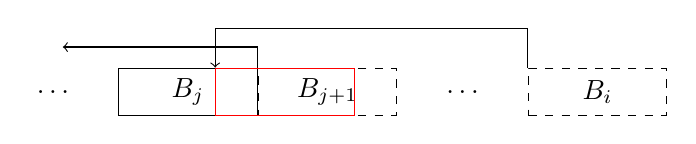
\begin{tikzpicture}[block/.style={draw,rectangle,minimum width=50pt,minimum height=1.7em},level/.style={sibling distance=40mm/#1},arrow/.style={draw=black, <-, shorten >=1pt}, edge from parent/.style={arrow}]
  \node[block,dashed] (block) {$B_i$};

  \node[left=5mm of block] (dots) {$\dots$};

  \node[block,left=5mm of dots,dashed] (source_r) {$B_{j+1}$};
  \node[block,left=0cm of source_r] (source_l) {$B_j$};
  \node[block,right=3.5em of source_l.west,red] (source) {};

  \node[left=5mm of source_l] (dots2) {$\dots$};

  \node[above=3mm of dots2] (dummy) {};


  \draw[->] (block.north west) -- ++(0,5mm) |- ([yshift=5mm,xshift=3.5em]source_l.north west) -- ([xshift=3.5em]source_l.north west);
  \draw[->] (source_r.north west) |- (dummy);
\end{tikzpicture}
\end{document}


